\documentclass[12pt,a4paper]{article}
\synctex=1
\usepackage[utf8]{inputenc}
\usepackage[margin=1cm]{geometry}
\usepackage{graphicx}
%\usepackage{verbatim}
\usepackage{amsmath}
\usepackage{amsfonts}
\usepackage{amssymb}
\usepackage{listings}
\usepackage{enumitem}
\usepackage{textcomp}
\usepackage{courier}
\usepackage{libertine}
\usepackage{pgfornament}
\usepackage{eso-pic}
\usepackage[hangul]{kotex}
\linespread{1.3}

\title{
	\centering
	\pgfornament[width=12cm,color=teal]{84}\\
	\vspace{1cm}
	\fontsize{50}{50} \selectfont {정보통신 수학 및 실습\\Homework}\\
		\pgfornament[width=12cm,color=teal]{88}\\
	\vfill}
\author{
	\LARGE
	\begin{tabular}{rl}
		\hline
		학번 : & 2016110056\\ 
		학과 : & 불교학부 \\
		이름 : & 박승원\\
		날짜 : & \today\\
		\hline
	\end{tabular}\vspace{2cm}
	\\

\includegraphics[width=0.5\textwidth]{logo.jpg}
	}
\date{}


\begin{document}
\maketitle
\pagenumbering{gobble}
\noindent
\lstset{language=matlab, columns=flexible, tabsize=4, frame=shadowbox, showstringspaces=false, breaklines=true, upquote=true, basicstyle=\normalsize}

\renewcommand{\thesubsubsection}{\alph{subsubsection})}
\renewcommand{\thesubsection}{\arabic{subsection}.}
\newpage

\section*{Chapter 10 Homework}
\subsection{Find the Fourier series of the following functions. } 
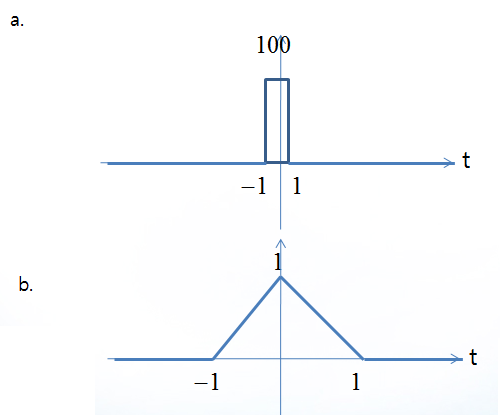
\includegraphics[width=\textwidth]{1.png}

even function 
\begin{gather*}
f(t) = a_0 + b_1 \cos t + b_2 \cos 2t + \cdots\\
a_0 = \int_{-\pi}^\pi f(t) dt = 0.2\\
b_n = \int_{-\pi}^\pi f(t)\cos(nt) dt
=\int_{-0.1}^{0.1}\cos(nt)dt
=\left[\frac{1}{n}\sin(nt)\right]_{-0.1}^{0.1}
=\frac{2}{n}\sin(0.1n) 
\end{gather*}
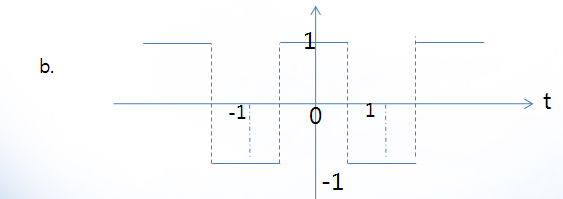
\includegraphics[width=\textwidth]{2.png}
\begin{gather*}
f(t) = a_0 + b_1 \cos \pi t + b_2 \cos 2\pi t+ \cdots\\
a_0 = \int_{-1}^1 f(t) = 0;
\end{gather*}
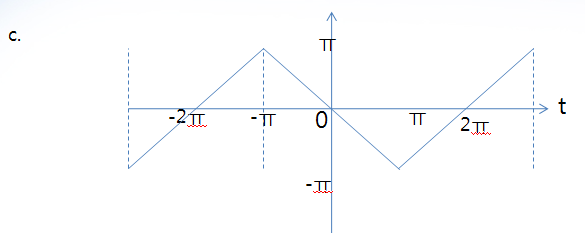
\includegraphics[width=\textwidth]{3.png}
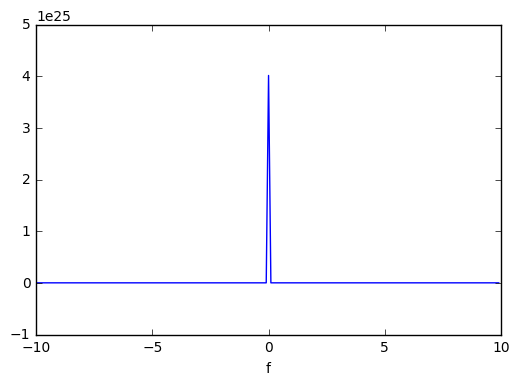
\includegraphics[width=0.5\textwidth]{4.png}
\end{document}
